\chapter{Part2: Characteristics of SISO feedback control systems}

\section{Design objectives}
In the design of a feedback control system, the following objectives have to be taken into account.
\subsection{Internal stability of the feedback control system}
For all bounded distrubances and inputs, the system response at every point inside the controll loop must be bounded. The difference between internal stability and input-output stability was established in the previous part. \\
\begin{factbox}
It is possible for a system to be internally unstable and yet to have a stable stansfer function, i.e to be input-output stable. This happens when the system has unstable hidden modesl.
\end{factbox}

\subsection{Robust stability}
If the plant deviate from a nominal model, \textbf{a set of models} is suitable for a better erepresentation of the plant.\\
The set of models could be generated, for example, by letting the model parameters very over their uncertainty intervals, with each parameter value defining a member of teh set.\\
For a controller design to be acceptable, \textbf{the feedback control system must be internally stable for every model in the set.} This property is referred to as \textit{Robust stability}.
\subsection{Tracking}
A good feedback control system must provide satisfactory steady-state and transient tracking. It is not usually possible to have good tracking for all possible reference input. That is the reason why response specifications are normally given in the presence of specific reference signals or classes of signals.

\subsection{Disturbance attenuation/rejection}
It is common to examine in some detail the response to polynomial disturbances and sinusoidal disturbances.

\section{Relative stability}
In the design of a control system, it is required that the system be stable. Further, it is necessary that the system has adequate relative stability. Consider the following figures.
\begin{figure}[H]
    \centering
    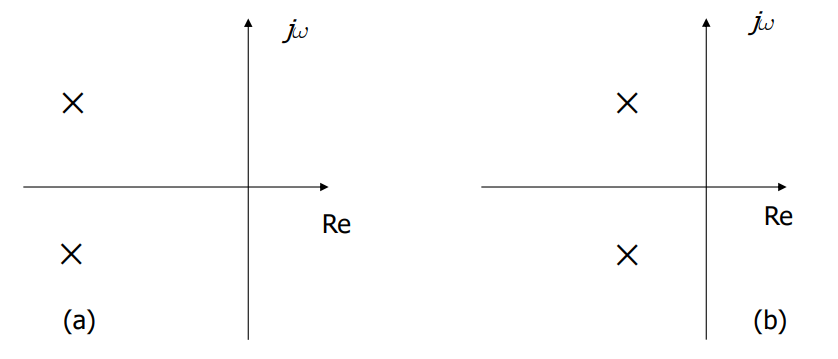
\includegraphics[width=0.75\textwidth]{relative-stability-01.png}
    \caption{The position of the poles of two system in \(S\)-plane; the system on the left represent a higher relative stability, since it is farther from the horizental axis, which is the verge of instability.}
    \label{fig:relative-stability-01}
\end{figure}

\begin{figure}[H]
    \centering
    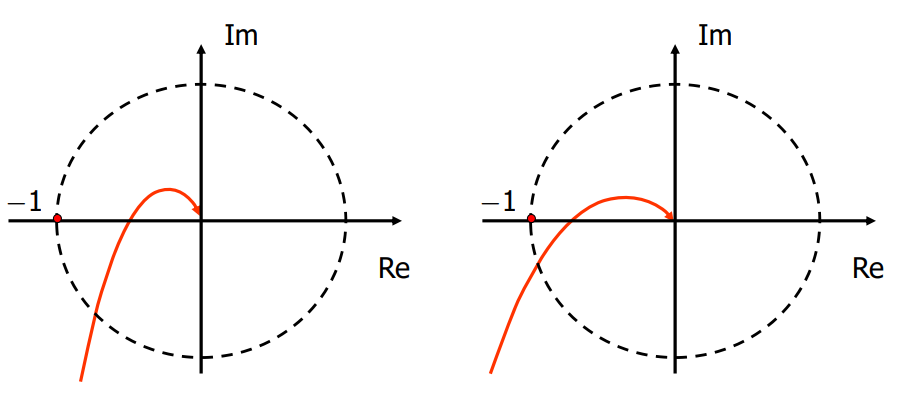
\includegraphics[width=0.75\textwidth]{relative-stability-02.png}
    \caption{The polar plot of the frequency response of two different systems; the system on the has a higher relative stability, since it has a large value of GM and PM.}
    \label{fig:relative-stability-02}
\end{figure}

In both figures, the system on represented on the
left is more stable than the system on the right. In the first figure, the system on the left is farther in the LHP, and in the second plot, the system on the left has a higher value of PM and GM.

The Nyquist criterion is defined in terms of the (-1, 0) point on the polar plot or the 0dB, -180° point on the Bode diagram or lag-magnitude-phase diagram. The proximity  of the \(GH(j\omega)\) locus to this stability pooint is a measure of relative stability. Consider the following transfer function and its polar diagram.
\[
G(s)H(s) = \frac{K}{s(\tau_1s +1)(\tau_2s+1)}
\]

\begin{figure}[H]
    \centering
    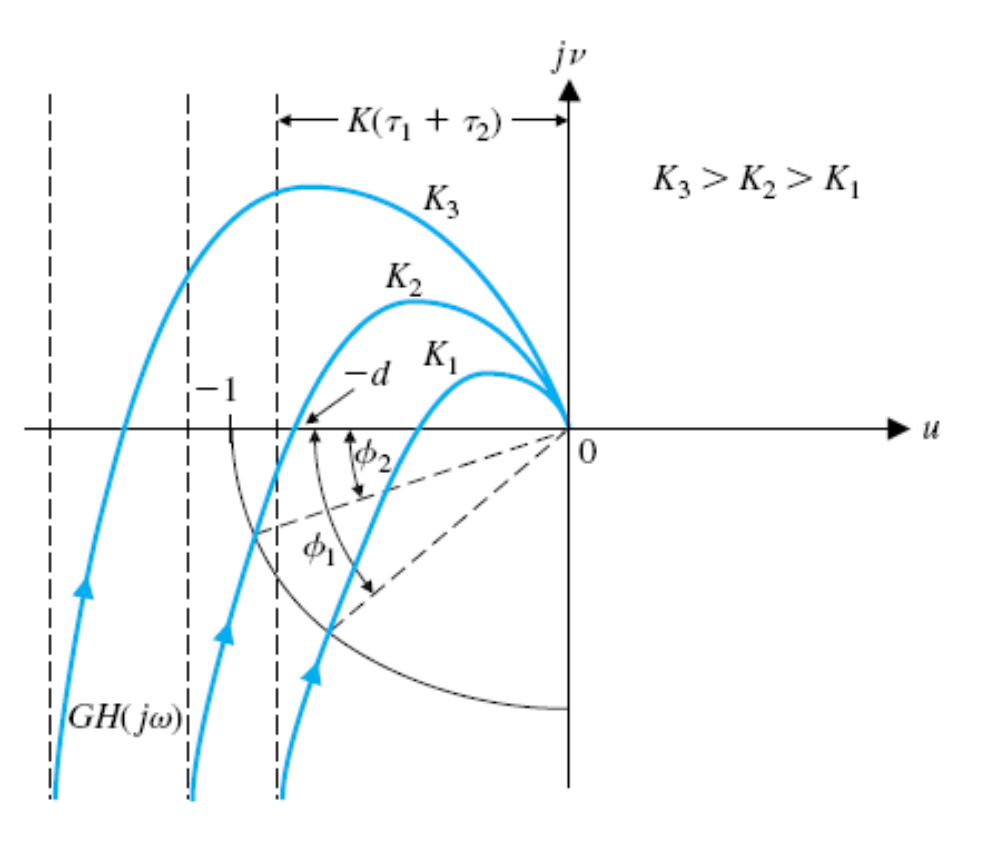
\includegraphics[width=0.5\textwidth]{relative-stability-03.png}
    \caption{The polar plot of the aforementioned transfer function for different value of gain \(K\).}
    \label{fig:relative-stability-03}
\end{figure}

FOR LOOP SHAPING LOOK AT THE NOTES MAKE FOR THE RESPONSE OF TEH LABS.

THIS PART CAN BE COMPLETED LATER IF IT IS NEEDED.
